
\section*{Results}
\vspace{-0.1cm}
We simulated $N= \,\,$\SI{5e5} synapses evolving as Kesten processes and recorded lifetime and weight distributions. First, we systemically tested the effect of the distribution parameters on lifetime and weight distributions. We found that within parameter ranges as for example used in the Kesten model of \textcite{Statman2014}, the variance of the multiplicative component $\sigma_a^2$ has negligible effect on lifetime and weight distributions. This allowed us to further reduce the Kesten model in complexity and allowed us to consider an autoregressive AR(1) process of the form
%
\begin{align}
  X_{n+1} = a\, X_n + b_n, \label{eq:ar1}
\end{align}
%
where $a \in (0,1)$ and $b_n \sim \mathcal{N}(\mu_b, \sigma_b^2)$ instead. The mean of the multiplicative component $\mu_a$ does affect both weight and lifetime distributions significantly and we found that biological realistic distributions arise when $\mu_a$ is close to $1$, as for in example in \cite{Statman2014} ($\mu_a \approx 0.99$). Indeed, in match with experimental data \cite{Loewenstein2015, Song2005} and predictions from network simulations \cite{Zheng2013} we found that for unbiased additive change ($\mu_b =0$), a power law like distribution of synaptic lifetimes emerges (Fig.~\ref{fig:lifetimes}A), while the distribution of spine sizes $X_{T_{\text{max}}}$ resembles a log-normal distribution.

\vspace{1cm}
\begin{overpic}[width=\columnwidth]%
  % 110, 133
  {figures/lifetimes_weights.pdf}
  %\put(32,\ylin){anisotropic}
  \put(1,28){\normalfont \textbf{A}}
  \put(52,28){\normalfont \textbf{B}}
\end{overpic}
\captionof{figure}[format=hang,indention=1cm]{Dynamical properties of network connectivity modelled by AR(1) process as in \eqref{eq:ar1}. \textbf{A} Lifetime distribution of synapses created at time step $T_{\text{init}}$ uniformly distributed in $[0, T_{\text{max}}]$. \textbf{B} Distribution of spine sizes $X_{T_{\text{max}}}$ at time step $X_{T_{\text{max}}}$ (grey) and log-normal fit (red). Parameters for both: $a=0.9987$, $\mu_b=0$, $\sigma_b^2=0.22$, $X_{\text{insert}}=0.1$, $X_{\text{prune}}=0.01$. \label{fig:lifetimes}}

\vspace{2.5cm}

%% \begin{center}\vspace{1cm}
%%   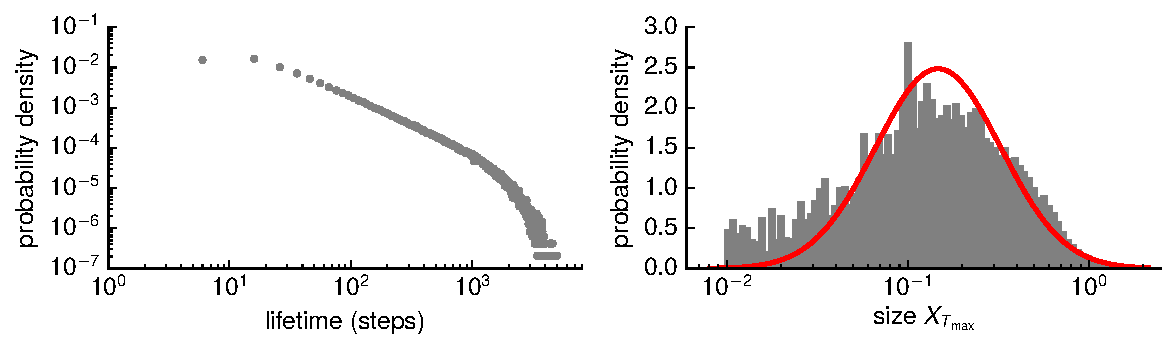
\includegraphics[width=\columnwidth]{%
%%     %% /home/fh/sci/lab/syn_lt/kesten_model/note_x/km_ca_rts_dd/img/lifetimes_weights.png}
%%     figures/lifetimes_weights.png}

%%   \captionof{figure}{}
%%   \label{fig:lifetimes}
%% \end{center}\vspace{1cm}
\begin{minipage}{\columnwidth}
We found the variance $\sigma_b^2$ of the additive component to have little effect on both the lifetime and spine size distributions. Interestingly however, the bias in the additive change affects both distributions significantly. A positive bias towards increases in size moves the tail of the lifetime distribution towards higher lifetimes (Fig.~\ref{fig:lifemub}A) while shifting the mean of the spine size towards higher values (Fig.~\ref{fig:lifemub}B). 

\vspace{1.5cm}
\begin{overpic}[width=\columnwidth]%
  % 110, 133
  {figures/lifetimes_weights_mub_compare_logweight.pdf}
  %\put(32,\ylin){anisotropic}
  \put(1,28){\normalfont \textbf{A}}
  \put(52,28){\normalfont \textbf{B}}
\end{overpic}
\captionof{figure}{The bias of additive change in size strongly affects both lifetime and weight distributions. \label{fig:lifemub}}
%\vspace{1.5cm}
\end{minipage}

%% This observation matches qualitatively with preliminary results from detailed network simulations in which a higher bias towards LTP resulted in similarly extended lifetimes.
